\documentclass{article}
\usepackage[table]{xcolor}
\usepackage{tikz}
\usetikzlibrary{automata,positioning,fit,arrows.meta,backgrounds,shapes.geometric}
\usepackage{tcolorbox}

\begin{document}

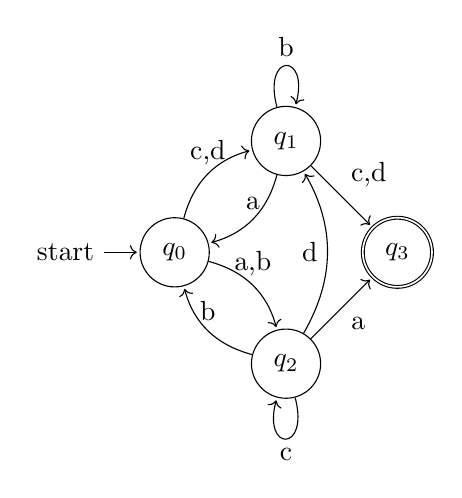
\begin{tikzpicture}[shorten >=1pt,node distance=2cm,on grid,auto] 
   \node[state,initial] (q_0)   {$q_0$}; 
   \node[state] (q_1) [above right=of q_0] {$q_1$}; 
   \node[state] (q_2) [below right=of q_0] {$q_2$}; 
   \node[state,accepting](q_3) [below right=of q_1] {$q_3$};
    \path[->]                                               
    (q_0) edge  [bend left, above] node  {c,d} (q_1)
          edge  [bend left, above] node [swap] {a,b} (q_2)
    (q_1) edge  node  {c,d} (q_3)
          edge [loop above] node {b} ()
          edge  [bend left, above] node   {a} (q_0)
    (q_2) edge  node [swap] {a} (q_3) 
          edge [loop below] node {c} ()
          edge [bend left, above] node {b} (q_0)
          edge [bend right,left] node {d} (q_1);
\end{tikzpicture}

\end{document}